\documentclass[a4paper,11pt,twocolumn]{article}
\usepackage[a4paper,left=1.5cm,right=1cm,top=2cm,bottom=2cm]{geometry}
\usepackage{amsmath}
\providecommand{\brak}[1]{\ensuremath{\left(#1\right)}}
\usepackage{listings}
\usepackage{xcolor}
\usepackage{tabularx}
\usepackage{graphicx}
\usepackage{watermark}
\usepackage{mathtools}
\graphicspath{{./figs}}
\usepackage[colorlinks,linkcolor={black},citecolor={blue!80!black},urlcolor={blue!80!black}]{hyperref}

\title{\textbf{\textsc{EC2018_46(FINDING AVERAGE VOLTAGE)}}}
\author{\textbf{\textit{ CHELIMI NANDINI (FWC22160)}}}

\begin{document}
\date{}
\maketitle
\tableofcontents

\section{PROBLEM}
\textbf{(GATE EC-2018)}
\textbf{Q.46} In the circuit shown below, a positive edge-triggered D flip-flop is used for sampling input data $ D_{in} $ using clock CK.The XOR gate outputs 3.3 volts for logic HIGH and 0 volts for logic LOW levels.The data bit and clock periods are equal and the value of $ \Delta T / T_{ck} $ = 0.15,where the parameters $ \Delta T $ and $ T_ck$ are shown in the figure.Assume that the Flip and the XOR gate are ideal.
%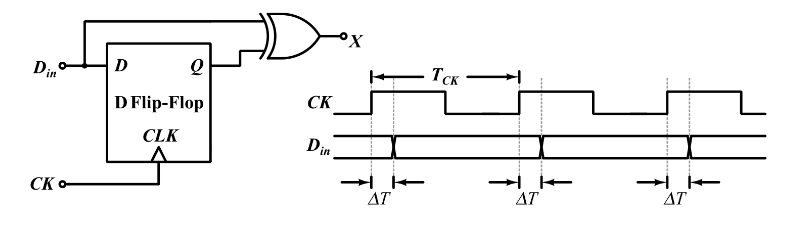
\includegraphics[scale=0.3]{figs/image.png}
\bigskip

\section{COMPONENTS}
	\begin{tabularx}{0.45\textwidth} {  
  | >{\centering\arraybackslash}X  
  | >{\centering\arraybackslash}X  
  | >{\centering\arraybackslash}X | } 
\hline 
\textbf{Component} &  \textbf{Value} & \textbf{Quantity}\\ 
\hline 
Arduino & UNO & 1 \\   
\hline 
Bread board & - & 1 \\ 
\hline 
IC & 7474 & 1 \\
\hline
Jumper wires & M-M & 20 \\ 
\hline 
LCD & 16X2 & 1\\ 
\hline 
Resistor & 1000ohms & 2\\ 
\hline
Led & - & 2\\
\hline
\end{tabularx}
\bigskip
\section{INTRODUCTION}
\par
Determining the average voltage at node $ X $ in a circuit that includes a positive edge-triggered D flip-flop and an XOR gate. The given parameters include the probability of input data bit (Din) transitions, the characteristics of the XOR gate, and the relationship between clock and data periods.The XOR gate outputs 3.3 volts for logic HIGH and 0 volts for logic LOW Level.\\
\newline
\textbf{Expression} : $ X = D_{in} \oplus Q $
\section{TRUTH TABLE}
Here truth table for output XOR
\begin{table}[!ht]
	\centering
	\begin{tabular}{ |c |c |c |c | }
		\hline
		\newline
		\textbf{time} & \textbf{$ D_{in} $} & \textbf{$ Q $} & \textbf{$ X $}\\
		\hline
		t1 & 1 & 0 & 1 \\
                t2 & 1 & 1 & 0 \\
		t3 & 0 & 1 & 1 \\
		t4 & 0 & 0 & 0 \\
		t5 & 1 & 0 & 1 \\
		
		\hline
        \end{tabular}
  \caption{}
\end{table}
\bigskip
\section{CALICULATIONS}
\textbf{Solution}: if the probability of input data bit($D_{in}$) transition in each clock period is 0.3.
$ V_{avg}$ = 0.85 * $ V_{high} $ * $ P_{high} $ + 0.15 *$V_{low}$*$P_{low} $\\
$ V_{avg}$ = 0.85 * 3.3 * 0.3 + 0.15 * 0 *0.7
$ V_{avg}$ = 0.8415

\section{ARDUINO CONNECTIONS}
\textbf{step1:} Connect the 5V pin of the Arduino to an extreme pin of the Breadboard.Let this pin be V cc .\\
\newline
\textbf{step2:} Connect the GND pin of the Arduino to the opposite extreme pin of the Breadboard.Let this pin be Ground.\\
\newline
\textbf{step3:} Connect Arduino pins to 7474 IC(DFlipflop) \\
\begin{table}[ht!] 
    \centering 
    \begin{tabular}{|c|c|c|c|c|c|c|c|c|} 
    \hline 
	    IC7474&ARDUINO  \\ 
         \hline 
	    pin1     &vcc \\
	    pin2(din)&pin3 \\
	    pin3(clk)&pin4 \\
	    pin4 & vcc \\
	    pin5(out) &pin5 \\
	    pin7 & GND \\
	    pin14 & vcc \\
         \hline 
    \end{tabular} 
\caption{} 
\end{table}
\\
\textbf{Step4:} We have to change $D_{in} $ manually from O(GND) to 1(VCC) using Jumpwires.Initially Dflipflop output consider as 0.\\
To see Dflipflop output we have to connect LED.LED(-ve to GND through 1kohm).7474 pin5 to LED(+ve).\\
\newline
\textbf{Step5:} Then $D_{in}$ and Dflipflop as input to Xor Output.Ouput can see through the LED(-ve to GND throungh 1kohms resistor).Arduino Pin6 LED(+ve).\\
\newline
\textbf{step6:} Connect LCD to Arduino \\
\begin{table}[ht!]
    \centering
    \begin{tabular}{|c|c|c|c|c|c|c|c|c|}
    \hline
            LCD&ARDUINO  \\
         \hline
	    pin1(Vss)&GND \\
	    pin2(Vcc)&Vcc \\
	    pin3(VEE)&220ohms(GND) \\
	    pin4(RS)& pin8 \\
            pin5(RW) &GND \\
            pin6(En)&pin9 \\
	    pin11(D4) & pin10 \\
	    pin12(D5)& pin11 \\
	    pin13(D6)& pin12\\
	    pin14(D7)& pin13\\
	    pin15(LED)&Vcc\\
	    pin16(LED)&GND\\
         \hline
    \end{tabular}
\caption{}
\end{table}
\\
\bigskip
\section{CODE}
\paragraph{}
	The arduino code can be downloaded from the below link.
\begin{center} 
%\fbox{\parbox{8.5cm}{\url{https://github.com/chelimi/ide/tree/main/ide}}} 
\end{center}
\bigskip
\section{RESULT}
According to the Probability Average Voltage will be displayed in LCD.
\end{document}
